\label{sec:fak_sol}
In this section the conformation of soluted FAK (FAK-SOL) for the \martini force field is investigated. Since the secondary structure of the two domains is fixed with the elastic network, the focus is on the FERM kinase interface.\\
\\
First the COM distances of F1 to the N-lobe ($d_\text{F1-N}$) and F2 to the C-lobe ($d_\text{F2-C}$) are considered. The two dimensional histogram of the distances reveals two different states ( \autoref{free:f2clf1nl}). Spot 1 refers to conformations, which are partially opened at the F2 - C-lobe interface, but close at the F1 - N-lobe interface. In contrast to this the conformations of spot 2 refers to states, in which F2 and the C-lobe gets closer while the distance between F1 and the N-lobe is increased. A comparison of the 3D structures induces, that spot 1 refers to a configuration, in which the kinase is slightly tilted against the FERM domain while it is line line for configurations associated with spot 2. During the simulation several transitions between the spots were obtained. At the end $47.4\%$ of the obtained distances were located in spot 1 and $52.6\%$ in spot 2.\\
However, there is only a minor effect upon the contact area (\autoref{free:ca}).  Spot 2 show a slightly larger mean value of $27.6\,\si{\nano\metre}^2$ in comparison to spot 1 ($27.1\,\si{\nano\metre}^2$).\\
\\
%
%
%
\begin{figure}
	\subcaptionbox{\label{free:f2clf1nl}}[0.49\textwidth]{
		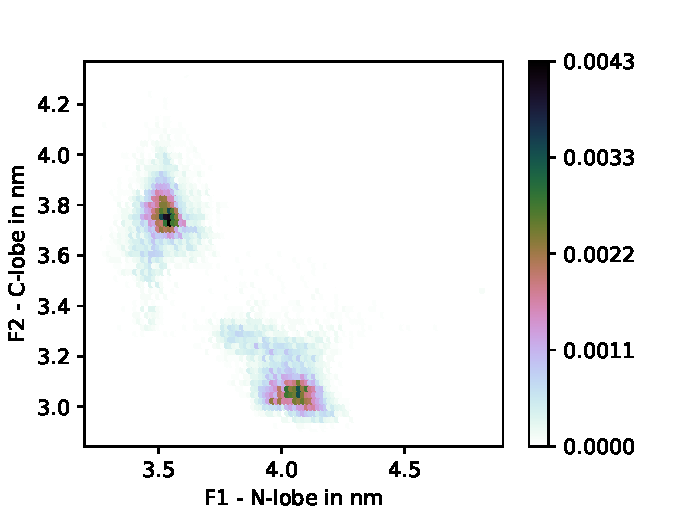
\includegraphics[height=5.2cm]{figures/results/free_f1f2}
	}\hfill%
	\subcaptionbox{\label{free:ca}}[0.49\textwidth]{
		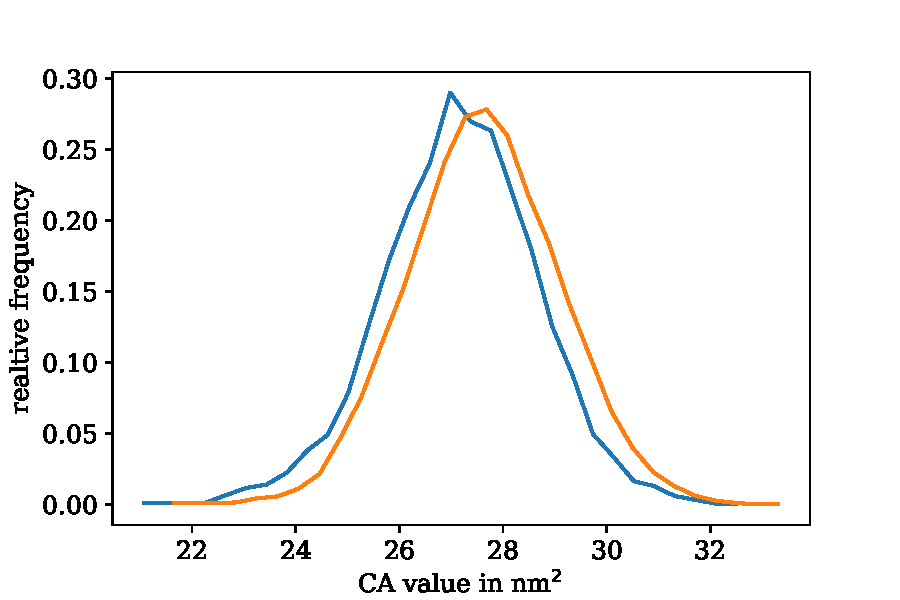
\includegraphics[height=5.2cm]{figures/results/free_ca}
	}%
	\nicecaption{Domain distances and contact area of FAK-SOL}{(\subref{free:f2clf1nl}): two dimensional hexbinning histogram of $d_\text{F1-N}$ and $d_\text{F2-C}$, which shows the two spots. (\subref{free:ca}): distribution of CA for the two spots.}
\end{figure}
%
%
%
A contact map of the interface between the FERM domain and the kinase for frames of spot 2 can be found in \autoref{free:contact}. Two contact areas can be identified at the FERM-kinase interface. The first one (area 1) is located between F1 and the N-lobe/activation loop. It shows i.e. contacts between \acid{Y}{576} and \acid{Y}{577} and residues of the FERM domain. The minimal distance in this area, occurring between residue \acid{H}{41} and \acid{Y}{576}, is $0.45\,\si{\nano\metre}$ with an RMSF value of $0.03\,\si{\nano\metre}$. This area reflects the burying of the activity regulating residues in closed state.\\
The second contact area (area 2) is located between F2 and the C-lobe. The spots occur around the residues \acid{Y}{180} and \acid{D}{200} of F2 as well as \acid{F}{596} and \acid{R}{665} of the C-lobe. The minimal distance in this area occurs between \acid{Y}{180} and \acid{F}{596} with $0.45\,\si{\nano\metre}$ and an RMSF value of $0.02\,\si{\nano\metre}$. Mutation experiments showed, that these two residues have an important effect upon the interface \autocite{structFAK}, which fits to the obtained contact.\\
The linker show contacts with both domains. The minimal distances in the marked areas occur between the autophosphorylation site \acid{Y}{397} and \acid{H}{58} of F1 ($0.45\,\si{\nano\metre}$, RMSF $0.03\,\si{\nano\metre}$) as well as \acid{Y}{397} and \acid{Y}{576} of the kinase ($0.50\,\si{\nano\metre}$, RMSF $0.10\,\si{\nano\metre}$). Furthermore several interactions occur between the residues in the linker, namely between \acid{S}{379} to \acid{V}{389} and \acid{T}{394} to \acid{I}{400} (area 5). Also in this spot the minimal distance occurs between \acid{Y}{397} and \acid{T}{386} ($0.52\,\si{\nano\metre}$, RMSF $0.04\,\si{\nano\metre}$). The density in this area induces that this region forms a ball, which is slightly plunged into the interface of the FERM domain and the kinase (regarding area 3 and area 4). These contacts support the thesis that autophosphorylation is prevented in closed conformation by a binding of the linker to the FERM domain \autocite{pap003}.\\ % TODO: smth like: they also give rise to an assumption what a release could look like oder so?
% TODO: write, why not presenting the second spot
%
%
%
\begin{figure}
	\centering
	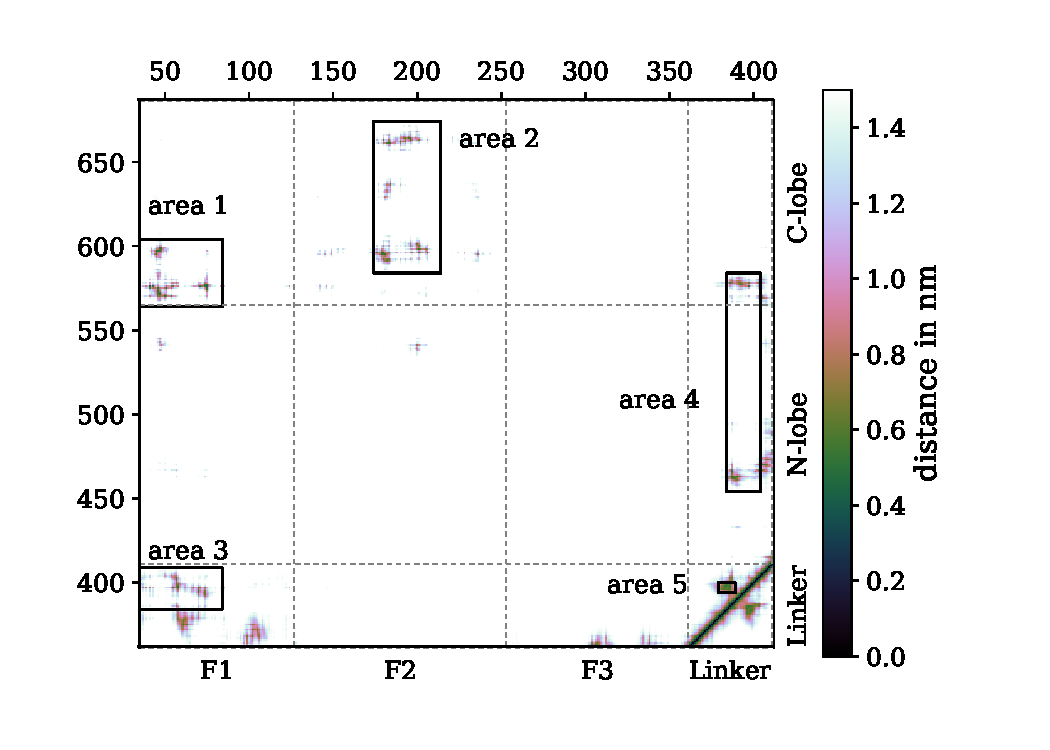
\includegraphics[width=.8\textwidth]{figures/results/contactmap_free}
	\nicecaption{Contactmap of FAK-SOL}{Contactmap of the FERM-kinase interface and the linker region.}
	\label{free:contact}
\end{figure}
%
%
%
